\documentclass[../PolyS1.tex]{subfiles}
\begin{document}

\section{Introduction : La loi des leviers ou balance d'Archimède}

\textbf{Loi 1 : }Des poids qui s'équilibrent à des distances égales sont égaux.
\begin{center}
\includegraphics{images/balance_archimede1}
\end{center}

\textbf{Loi 2 : }Des poids inégaux s'équilibrent \`a des distances inégales et le plus grand sera situé \`a la plus petite distance.


\textbf{Loi 3 : }Des poids quelconques s'équilibrent \`a des distances inversement proportionnelles \`a ces poids.\\
\begin{center}
\includegraphics{images/balance_archimede2}
\end{center}
%
%\gen{On s'intéresse \à des systémes virtuels représentés par un nombre finis de points (2 ou 3) affectés individuellement d'une masse (poids, force). On peut alors concevoir le barycentre comme la moyenne pondérée des forces en présence...}
%
\paragraph{Illustration}

Si un point A est affecté d'un poids de 2 et un point B d'un poids de 3. On considére leur barycentre G. 

\begin{center}
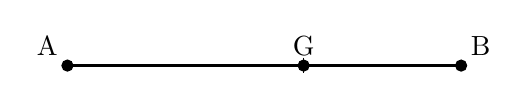
\begin{tikzpicture}
    % Dessin du segment AB avec des points aux extrémités
    \draw[thick] (0,0) -- (5,0);
    \filldraw (0,0) circle (2pt) node[above left] {A};
    \filldraw (5,0) circle (2pt) node[above right] {B};

    % Marque pour le point G
    \filldraw (3,0) circle (2pt) node[above] {G};
    \draw (3,0.1) -- (3,-0.1); % Petite marque verticale à G
\end{tikzpicture}
\end{center}

D'après la loi des leviers, $\dfrac{GA}{GB}=3/2$ ou encore $2GA=3GB$. Les vecteurs $\overrightarrow{GA}$ et $\overrightarrow{GB}$ étant \textbf{colinéaires} et de sens contraire, $2\overrightarrow{GA}=-3\overrightarrow{GB}$. Soit : $$2\overrightarrow{GA}+3\overrightarrow{GB}=\vec0$$
%\newpage
%%%%%
%
\section{Barycentres de deux points pondérés}
\subsection{Définitions}

Les définitions et propriétés qui suivent sont valables seulement dans le plan ou l'espace usuels.
\medskip

\begin{Def}\textbf{Barycentre}
    \vspace{1em}

$A$ et $B$ sont des points, $a$ et $b$ sont des nombres réels tels que : $a+b\neq0$.

Le {\bf barycentre} des points pondérés $(A,a)$ et $(B,b)$ est le point $G$ défini par : $$a\,\overrightarrow{GA}+b\,\overrightarrow{GB}=\overrightarrow0.$$

\end{Def}

%\begin{Rem}
Pour placer le point $G$, on peut utiliser l'égalité vectorielle : $\overrightarrow{AG}=\dfrac{b}{a+b}\overrightarrow{AB}.$

%\end{Rem}
\hfill\break
\hrule
\hfill\break

\exo[1]{Premier barycentre}

Soient deux points quelconques $A$ et $B$.
 Construire le barycentre du syst\`eme $\left\{(A,3);(B,1)\right\}$.

\hfill\break
\hrule
\hfill\break

%
%\begin{Rem}
On convient d'écrire : 
\begin{center}
$G$ bar 
$\begin{array}{c|c} A&B\\\hline a&b\end{array}$.
\end{center}
%\end{Rem}
%


\newpage


\subsection{Propriétés}

\begin{Prop}\textbf{Propriété fondamentale}
    \vspace{1em}

Soit $G$ le barycentre du syst\`eme $\left\{(A,a);(B,b)\right\}$. Pour tout point $M$ : $$a\,\overrightarrow{MA}+b\,\overrightarrow{MB}=(a+b)\,\overrightarrow{MG}.$$

\end{Prop}
\hfill\break
\hrule
\hfill\break

\exo[1]{Propiété}
Démontrer la propriété précédente en utilisant la relation de Chasles \`a partir de la définition de $G$.


%\newpage
%%%%%

\hfill\break
\hrule
\hfill\break

\exo[1]{Coordonnées}
On se place dans un rep\`ere $(O;\overrightarrow{i};\overrightarrow{j})$ du plan. On consid\`ere les points $A(1;2)$ et $B(-2;4)$.

Déterminer les coordonnées de $G$ barycentre du syst\`eme $\left\{(A,3);(B,1)\right\}$.

\hfill\break
\hrule
\hfill\break



\begin{Prop}\textbf{Multiplication par un scalaire}
    \vspace{1em}

Si $k$ est un réel non nul, le barycentre de $(A,a)$ et $(B,b)$ est aussi celui de $(A,ka)$ et $(B,kb)$.
\end{Prop}

%\begin{Rem}
On utilise cette propriété pour simplifier l'égalité $a\overrightarrow{GA}+b\overrightarrow{GB}=\overrightarrow0$ afin de faciliter la construction géométrique de $G$.
%\end{Rem}

\hfill\break
\hrule
\hfill\break

\exo[2]{Deux points}
Soient deux points quelconques $A$ et $B$.

 Construire le barycentre du syst\`eme $\left\{\left(A,\frac{2}{7}\right); \left(B,\frac{-1}{7}\right)\right\}$.


\hfill\break
\hrule
\hfill\break

%\vspace{3cm}

\newpage


\exo[1]{Milieu}
Soient deux points quelconques $A$ et $B$, et $I$ le milieu de $[AB]$. Donner plusieurs syst\`emes $\left\{(A,a); (B,b)\right\}$ dont $I$ est le barycentre.

\hfill\break
\hrule
\hfill\break

\begin{Prop}\textbf{Position de $G$}
    \vspace{1em}

Si $G$ est un barycentre du système $\left\{(A,a); (B,b)\right\}$, alors 
 \begin{enumerate}%[$\bullet$]
 \item $G$ est sur la droite $(AB)$ : $G\in(AB)$.
 \item Si $a$ et $b$ sont de m\^ eme signe, alors $G$ est sur le segment $[AB]$ : $G\in[AB]$.
 \item Si $a$ et $b$ sont de signe contraire, alors $G\notin[AB]$.
 %\item Si $\abs{a} >\abs{b}$, alors $G$ est \og plus pr\`es\fg\ de $A$ que de $B$.
 \end{enumerate}
\end{Prop}
%\newpage
%%%%%





\subsection{QCM}


\begin{center}
\textbf{Chaque question peut avoir une ou plusieurs bonnes réponses.}
\end{center}

\begin{enumerate}[label=\textbf{Q\arabic*.}]

\item Soient deux points \( A \) et \( B \). Le barycentre \( G \) de \( (A,1) \) et \( (B,1) \) est :
\begin{multicols}{2}
\begin{itemize}
    \item[1.] Le point \( A \)
    \item[2.] Le point \( B \)
    \item[3.] Le milieu du segment \( [AB] \)
    \item[4.] Le point tel que \( \overrightarrow{AG} = \dfrac{1}{2} \overrightarrow{AB} \)
\end{itemize}
\end{multicols}

\item Le barycentre \( G \) de \( (A,2), (B,3) \) vérifie :
\begin{multicols}{2}
\begin{itemize}[itemsep=1em]
    \item[1.] \( \overrightarrow{AG} = \dfrac{3}{5} \overrightarrow{AB} \)
    \item[2.] \( \overrightarrow{BG} = \dfrac{2}{5} \overrightarrow{BA} \)
    \item[3.] \( \overrightarrow{GA} = \dfrac{3}{5} \overrightarrow{BA} \)
    \item[4.] \( \overrightarrow{GB} = \dfrac{2}{5} \overrightarrow{AB} \)
\end{itemize}
\end{multicols}

\item Le point \( G \), barycentre de \( (A,2), (B,-2) \), est :
\begin{multicols}{2}
\begin{itemize}
    \item[1.] Le point \( A \)
    \item[2.] Le point \( B \)
    \item[3.] Situé sur la droite \( (AB) \)
    \item[4.] Non défini (car somme des poids nulle)
\end{itemize}
\end{multicols}

\end{enumerate}








\newpage


\section{Barycentre de trois points pondérés}
\subsection{Définition et propriété fondamentale}

\begin{Def}\textbf{Barycentre de trois points}
\vspace{1em}

$A, B, C$ sont des points, $a, b, c $ sont des nombres réels tels que : $a+b+c\neq0$.

Le {\bf barycentre} du syst\`eme $\left\{(A,a);(B,b);(C,c)\right\}$ est le point $G$ défini par : $$a\,\overrightarrow{GA}+b\,\overrightarrow{GB}+c\,\overrightarrow{GC}=\overrightarrow0.$$
\end{Def}

\begin{Prop}\textbf{Barycentre}
    \vspace{1em}

Soit $G$ le barycentre du syst\`eme $\left\{(A,a);(B,b);(C,c)\right\}$. Pour tout point $M$ : $$a\overrightarrow{MA}+b\overrightarrow{MB}+c\overrightarrow{MC}=(a+b+c)\overrightarrow{MG}.$$
\end{Prop}

%\begin{Rem}
On convient d'écrire : 
\begin{center}
    
$G$ bar $\begin{array}{c|c|c} A&B&C\\\hline a&b&c\end{array}$.
\end{center}
%\end{Rem}

\subsection{Propriétés}

\begin{Prop}\textbf{Coplanarité}
    \vspace{1em}

Le barycentre de trois points pondérés non alignés de l'espace appartient au plan déterminé par ces trois points.
\end{Prop}

\begin{Prop}\textbf{Simplification}
    \vspace{1em}

 On peut multiplier ou diviser par un m\^eme réel non nul tous les coefficients de plusieurs points pondérés sans changer leur barycentre.
\end{Prop}

\begin{Prop}\textbf{Barycentre partiel ou associativité}
    \vspace{1em}

On ne change pas le barycentre de 3 points pondérés si l'on remplace 2 points pondérés par leur barycentre (sous réserve d'existence) affecté de la somme de leurs coefficients.
\end{Prop}

\underline{Autrement dit :} Si 

\noindent $G$ est le barycentre du syst\`eme $\left\{(A,a);(B,b);(C,c)\right\}$ ($a+b+c\neq0$),\newline 
et $H$ le barycentre du syst\`eme $\left\{(A,a);(B,b)\right\}$ ($a+b\neq0$),\newline

alors $G$ est le barycentre du syst\`eme $\left\{(H,a+b);(C,c)\right\}$.
\hfill\break
%


\hfill\break
\hrule
\hfill\break


\exo[2]{Système barycentrique}
On cherche \`a construire le barycentre $G$ du syst\`eme $\left\{(A,2);(B,1);(C,4)\right\}$. \begin{enumerate}\item Par exemple, on construit le barycentre $H$ du syst\`eme $\left\{(A,2);(B,1)\right\}$ : $\overrightarrow{AH}=\dfrac{1}{3}\overrightarrow{AB}$.
\item On construit le barycentre $G$ du syst\`eme $\left\{(H,3);(C,4)\right\}$ : $\overrightarrow{HG}=\dfrac{4}{7}\overrightarrow{HC}$.\\

\end{enumerate}




\begin{center}
\begin{tikzpicture}
    % Définition des points
    \coordinate (A) at (0,0);
    \coordinate (B) at (3,1);
    \coordinate (C) at (4,-3);
    \coordinate (H) at (1,0.33);
    \coordinate (G) at (2.71,-1.57);

    % Dessin des segments
    \draw (A) -- (B);
    \draw (B) -- (C);
    \draw[dashed] (H) -- (C);

    % Étiquettes des points
    \node[left] at (A) {A};
    \node[right] at (B) {B};
    \node[right] at (C) {C};
    \node[above] at (H) {H};
    \node[above] at (G) {G};

    % Petits "+" pour marquer les points
    \foreach \p in {A,B,C,H,G} {
        \node at (\p) {+};
    }

\end{tikzpicture}
\end{center}

\hfill\break
\hrule
\hfill\break

%\end{center}

\exo[2]{Rectangle}

Soit $ABCD$ un rectangle et $G$ bar $\begin{array}{c|c|c|c} A&B&C&D\\\hline 1&1&1&3\end{array}$.\newline En considérant $I$ bar $\begin{array}{c|c} A&B\\\hline 1&1\end{array}$ puis $J$ bar $\begin{array}{c|c} C&D\\\hline 1&3\end{array}$, montrer que $G$ bar $\begin{array}{c|c} I&J\\\hline 1&2\end{array}$, construire $G$.\\

\hfill\break
\hrule
\hfill\break
%\vspace{6cm}

\newpage


\exo[2]{Triangle}

Soit $ABC$ un triangle ; $I$ et $J$ sont les milieux respectifs des c\^otés $[AB]$ et $[AC]$.

$D$ est le barycentre du syst\`eme $\left\{(A,3);(B,2)\right\}$ ; $G$ est celui de $\left\{(A,3);(B,2);(C,1)\right\}$.

\begin{enumerate}
\item Construire le point $D$.
\item Démontrer que $G$ est le barycentre du syst\`eme $\left\{(D,5);(C,1)\right\}$ et également celui de $\left\{(I,2);(J,1)\right\}$\newline (indication : $G$ bar $\begin{array}{c|c|c} A&B&C\\\hline 3&2&1\end{array}\Longleftrightarrow G$ bar $\begin{array}{c|c|c|c} A&A&B&C\\\hline 2&1&2&1\end{array}$).
\item En déduire que les droites $(IJ)$ et $(CD)$ sont sécantes en $G$.\\
\end{enumerate}

\hfill\break
\hrule
\hfill\break
%
%\newpage
%%%%%
\subsection{Isobarycentre de trois points}

\begin{Def}\textbf{Isobarycentre}
    \vspace{1em}

Notons $A, B, C$ trois points.\\

Le {\bf barycentre} du syst\`eme $\left\{(A,1);(B,1);(C,1)\right\}$ est appelé {\bf isobarycentre} des points $A, B, C$ et : $$\overrightarrow{GA}+\overrightarrow{GB}+\overrightarrow{GC}=\overrightarrow0.$$
\end{Def}

\begin{Def}\textbf{Centre de gravité}
    \vspace{1em}

{\bf Le centre de gravité} d'un triangle  $ABC$ est l'isobarycentre des sommets.\\
\end{Def}


\hfill\break
\hrule
\hfill\break

\exo[2]{Associativité}
Soit $ABC$ un triangle. \`A l'aide du théor\`eme d'associativité, construire le centre de gravité du triangle $ABC$.\\

\hfill\break
\hrule
\hfill\break
%
%\newpage
%%%%%
%

\newpage


\subsection{QCM}

\begin{center}
\textbf{Chaque question peut avoir une ou plusieurs bonnes réponses.}
\end{center}



\begin{enumerate}[label=\textbf{Q\arabic*.}]

\item Le barycentre de trois points pondérés \( A(a), B(b), C(c) \), avec \( a+b+c \neq 0 \), est bien défini si :
\begin{multicols}{2}
\begin{itemize}
    \item[1.] Tous les poids sont positifs
    \item[2.] Les points sont alignés
    \item[3.] Les poids ne sont pas tous nuls
    \item[4.] La somme des poids est non nulle
\end{itemize}
\end{multicols}

\item Dans un repère, soient \( A(0,0), B(2,0), C(0,3) \). Le centre de gravité \( G \) du triangle \( ABC \) a pour coordonnées :
\begin{multicols}{2}
\begin{itemize}
    \item[1.] \( (1,1.5) \)
    \item[2.] \( (1,1) \)
    \item[3.] \( (2,3) \)
    \item[4.] \( \left( \dfrac{2}{3}, 1 \right) \)
\end{itemize}
\end{multicols}

\item L'isobarycentre de \( A, B, C \) correspond à :
\begin{multicols}{2}
\begin{itemize}
    \item[1.] Le barycentre de \( (A,1), (B,1), (C,1) \)
    \item[2.] Le point d'intersection des médianes
    \item[3.] Le centre de gravité
    \item[4.] Le point le plus proche de \( A \)
\end{itemize}
\end{multicols}

\item Soient \( A(1,1), B(3,5), C(4,-2) \). Le barycentre \( G \) de \( (A,2), (B,1), (C,1) \) a pour coordonnées :
\begin{multicols}{2}
\begin{itemize}
    \item[1.] \( (2.25, 1.5) \)
    \item[2.] \( (2.25, 1) \)
    \item[3.] \( (3, 1) \)
    \item[4.] \( \left( \dfrac{2 \cdot 1 + 1 \cdot 3 + 1 \cdot 4}{4}, \dfrac{2 \cdot 1 + 1 \cdot 5 + 1 \cdot (-2)}{4} \right) \)
\end{itemize}
\end{multicols}

\item Si \( G \) est le barycentre de \( (A,1), (B,2), (C,3) \), alors :
\begin{itemize}
    \item[1.] \( \overrightarrow{AG} + \overrightarrow{BG} + \overrightarrow{CG} = \overrightarrow{0} \)
    
    \item[2.] \( G \) est plus proche de \( C \) que de \( A \)
    \item[3.] \( G \) appartient au plan défini par \( A, B, C \)
    \item[4.] \( G \) est le centre de gravité du triangle \( ABC \)
\end{itemize}

\end{enumerate}




\section{Centre d'inertie d'une plaque homog\`ene}

\subsection{Principes de base}

\underline{Le principe du triangle}

Le centre d'inertie d'une plaque triangulaire est le centre de gravité du triangle.

\underline{Le principe de symétrie}
\begin{enumerate}%[\ding{51}]
\item Si la plaque admet un centre de symétrie $I$, le centre d'inertie est le point $I$.
\item Si la plaque admet un axe de symétrie $\Delta$, le centre d'inertie est sur la droite $\Delta$.
\end{enumerate}

\underline{Le principe de juxtaposition}
\hfill\break

\begin{minipage}{0.6\linewidth}
Le centre d'inertie $I$ de la plaque $\cal P$ est le barycentre du syst\`eme $\{(I_1,m_1),(I_2,m_2)\}$ o\`u la plaque ${\cal P}_1$ a pour masse $m_1$, pour aire $S_1$ et pour centre d'inertie $I_1$ et ${\cal P}_2$ a pour masse $m_2$, pour aire $S_2$ et pour centre d'inertie $I_2$.

\textcolor{red}{\ding{43} Les aires étant proportionnelles aux masses alors le point $I$ est le barycentre du système $\{(I_1,S_1);(I_2,S_2)\}$.\\
}
\end{minipage}
\begin{minipage}{0.4\linewidth}

\begin{center}
\includegraphics[height=5cm]{images/plaque1.png}
\end{center}

\end{minipage}

%\newpage
%%%%%%
\subsection{Exemples de plaques enti\`eres}
%
%\paragraph{Exemple 1\\}

\hfill\break
\hrule
\hfill\break

\exo[2]{Trapèze}

Dans une plaque métallique d'épaisseur constante, on a découpé le trap\`eze rectangle schématisé ci-dessous.\\
%
\begin{center}
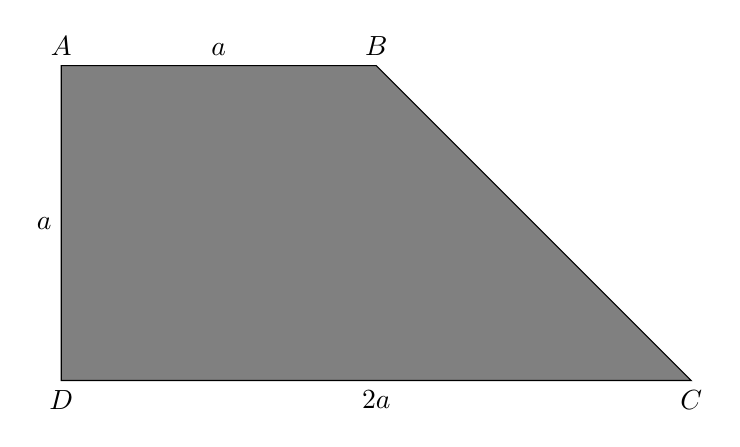
\begin{tikzpicture}

% Remplissage du quadrilatère
\fill[gray] (0,0) -- (8,0) -- (4,4) -- (0,4) -- cycle;

% Contour du quadrilatère
\draw (0,0) -- (8,0) -- (4,4) -- (0,4) -- cycle;

% Noms des sommets
\node[below] at (0,0) {$D$};
\node[above] at (0,4) {$A$};
\node[above] at (4,4) {$B$};
\node[below] at (8,0) {$C$};

% Étiquetage des longueurs
\node[left] at (0,2) {$a$};
\node[above] at (2,4) {$a$};
\node[below] at (4,0) {$2a$};

\end{tikzpicture}
\end{center}

%
\begin{enumerate}
\item Déterminer la position du centre d'inertie $I$.
\item $I$ est-il l'isobarycentre des sommets ?\\
\end{enumerate}



% %%SOLUTION
% \begin{Sol}
% %\begin{minipage}{0.6\linewidth}
% \begin{enumerate}
% \item $I$ est le barycentre du syst\`eme $\begin{array}{c|c} G_1&G_2\\\hline a^2&a^2/2\end{array}=\begin{array}{c|c} G_1&G_2\\\hline 2&1\end{array}$ o\`u $G_1$ est le centre du carré $ABED$ et $G_2$ le barycentre du triangle $BCE$ (intersections des médianes). Finalement, $\overrightarrow{G_1I}=\dfrac{1}{3}\overrightarrow{G_1G_2}$
% \item $I$ n'est pas l'isobarycentre des sommets. En effet, l'isobarycentre des sommets est $$\text{bar }\begin{array}{c|c|c|c} A&B&C&D\\\hline 1&1&1&1\end{array}=\text{bar }\begin{array}{c|c} K&J\\\hline 2&2\end{array}$$
% Il s'agit du milieu de $[KJ]$. ce n'est pas le point $I$ (en fait, il faudrait que la plaque $ABCD$ admet un centre de symétrie...).
% \end{enumerate}
% %\end{minipage}\hspace{1cm}
% \begin{minipage}{0.3\linewidth}
% \begin{center}
% \begin{tikzpicture}[scale=0.5]

% % Remplissage du quadrilatère
% \fill[gray!30] (0,0) -- (8,0) -- (4,4) -- (0,4) -- cycle;

% % Contour du quadrilatère
% \draw (0,0) -- (8,0) -- (4,4) -- (0,4) -- cycle;

% % Diagonales (pointillées)
% \draw[dotted] (0,0) -- (4,4);
% \draw[dotted] (0,4) -- (4,0);

% % Médianes (pointillées)
% \draw[dotted] (4,0) -- (6,2);
% \draw[dotted] (4,4) -- (6,0);

% % Segment G1G2 (pointillé)
% \draw[dotted] (2,2) -- (5.4,1.3);

% % Points marqués avec "+"
% \node at (6,2) {\bf +};
% \node at (3.2,1.8) {\bf +};
% \node at (0,2) {\bf +};

% % Légendes des sommets
% \node[below] at (0,0) {$D$};
% \node[above] at (0,4) {$A$};
% \node[above] at (4,4) {$B$};
% \node[below] at (8,0) {$C$};
% \node[below] at (4,0) {$E$};

% % Légendes des points
% \node[above] at (2,2) {$G_1$};
% \node[above] at (6,0.5) {$G_2$};
% \node[above left] at (0,2) {$K$};
% \node[above] at (3.4,1.7) {$I$};
% \node[above] at (6,2) {$J$};

% % Étiquetage des longueurs
% \node[above] at (2,4) {$a$};
% \node[below] at (2,0) {$a$};
% \node[below] at (6,0) {$a$};

% \end{tikzpicture}
% \end{center}
% \end{minipage}

% %\end{minipage}
% \end{Sol}

%%\vspace{4cm}
%

\hfill\break
\hrule
\vspace{1em}

\newpage

\exo[2]{Côtés}

Une plaque est formée de deux carrés $C_1$ et $C_2$. Son centre d'inertie I est deux fois plus pr\`es de $O_1$ que de $O_2$.\\
\begin{center}
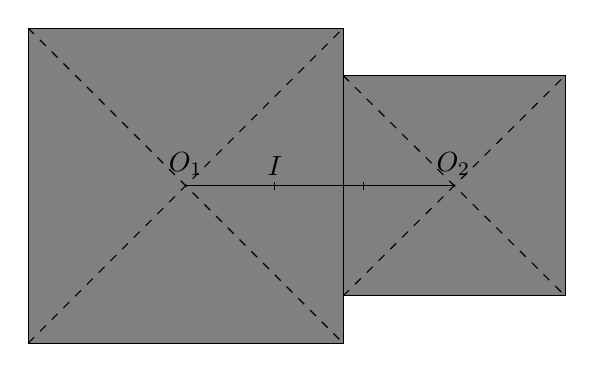
\begin{tikzpicture}

% Remplissage des deux polygones
\fill[gray] (0,0) -- (4,0) -- (4,4) -- (0,4) -- cycle;
\fill[gray] (4,0.6) -- (4,3.4) -- (6.82,3.4) -- (6.82,0.6) -- cycle;

% Contour des polygones
\draw (0,0) -- (4,0) -- (4,4) -- (0,4) -- cycle;
\draw (4,0.6) -- (4,3.4) -- (6.82,3.4) -- (6.82,0.6) -- cycle;

% Lignes pointillées
\draw[dashed] (0,0) -- (4,4);
\draw[dashed] (0,4) -- (4,0);
\draw[dashed] (4,0.6) -- (6.82,3.4);
\draw[dashed] (4,3.4) -- (6.82,0.6);

% Segments pleins
\draw (2,2) -- (5.4,2);
\draw (3.13,2.05) -- (3.13,1.95);
\draw (4.26,2.05) -- (4.26,1.95);

% Noms des points
\node[above] at (2,2) {$O_1$};
\node[above] at (5.4,2) {$O_2$};
\node[above] at (3.13,2) {$I$};

\end{tikzpicture}
\end{center}


Comparer les longueurs du c\^oté de $C_1$ et du c\^oté de $C_2$.\\


\hfill\break
\hrule
\hfill\break

% \begin{Sol}
% Notons $a,b$ les longueurs respectives des carré de centre $O_1$ et $O_2$. L'énoncé nous dit que $I$ bar $\begin{array}{c|c} O_1&O_2\\\hline 2&1\end{array}$. Par ailleurs, $I$ bar $\begin{array}{c|c} O_1&O_2\\\hline a^2&b^2\end{array}$. Du fait de l'unicité du barycentre d'un syst\`eme pondéré et donc de la proportionnalité des poids, on déduit que $$\dfrac{2}{1}=\dfrac{a^2}{b^2}\iff a=b\sqrt 2$$
% \end{Sol}
%%%%%%
%
\subsection{Point méthode : plaque évidée}
%
\begin{minipage}{0.6\linewidth}
On considère la plaque {\bf homog\`ene} $\cal P$ ci-dessous, o\`u la partie grisée est la matiére, et la partie claire un évidement :\\

On définit $\cal P$ \`a partir de la plaque homog\`ene compl\`ete ${\cal P}_1$, de centre d'inertie $I_1$, de masse $m_1$, d'aire $S_1$ évidée de la plaque homogène ${\cal P}_2$, de centre d'inertie $I_2$, de masse $m_2$, d'aire $S_2$ (les aires sont proportionnelles aux masses).

\textcolor{red}{\ding{43} Le centre d'inertie de $\cal P$ est le point $G$ barycentre du syst\`eme $\{(I_1,S_1);(I_2,-S_2)\}$.\\}
\end{minipage}
\begin{minipage}{0.4\linewidth}
\begin{center}
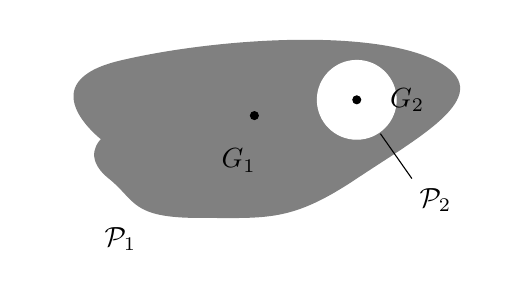
\begin{tikzpicture}

% Courbe fermée
\fill[gray] plot[smooth, tension=1] coordinates {(0.75,1) (1,2) (5,2) (4,0.5) (2,0) (0.85,0.5) (0.75,1)} -- cycle;

% Cercle blanc
\fill[white] (4,1.5) circle (0.5);
\draw[white] (4,1.5) circle (0.5);

% Points noirs
\filldraw (2.7,1.3) circle (0.05);
\filldraw (4,1.5) circle (0.05);

% Labels
\node[below] at (1,0) {${\cal P}_1$};
\node[below] at (5,0.5) {${\cal P}_2$};
\node[below] at (2.5,1) {$G_1$};
\node[right] at (4.3,1.5) {$G_2$};

% Petite ligne
\draw[thin] (4.3,1.07) -- (4.7,0.5);

\end{tikzpicture}
\end{center}
\end{minipage}

\newpage

\subsection{Exemples de plaques évidées}


\exo[2]{Plaque homogène}

On consid\`ere la plaque homog\`ene ci-dessous :\\

\begin{center}
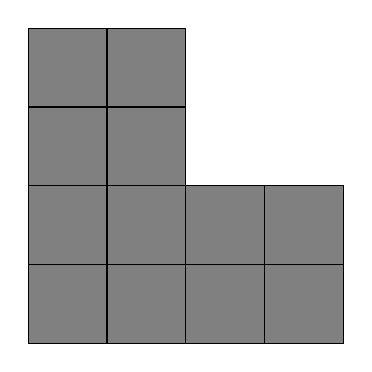
\begin{tikzpicture}

% Remplissage du polygone
\fill[gray] (0,0) -- (4,0) -- (4,2) -- (2,2) -- (2,4) -- (0,4) -- cycle;

% Contour du polygone
\draw (0,0) -- (4,0) -- (4,2) -- (2,2) -- (2,4) -- (0,4) -- cycle;

% Lignes intérieures verticales
\draw[thin] (1,0) -- (1,4);
\draw[thin] (2,0) -- (2,2);
\draw[thin] (3,0) -- (3,2);

% Lignes intérieures horizontales
\draw[thin] (0,1) -- (4,1);
\draw[thin] (0,2) -- (2,2);
\draw[thin] (0,3) -- (2,3);

\end{tikzpicture}
\end{center}

Déterminer le centre d'inertie $G$ de la plaque en utilisant la méthode directe (juxtaposition de deux plaques pleines) puis en utilisant la méthode avec un évidement (plaque compléte à laquelle on enl\`eve une plaque).

%
% \begin{Sol}
% \begin{minipage}{0.6\linewidth}
% \begin{itemize}
% \item {\bf Méthode directe : } soient $G_1$ le centre d'inertie de la plaque grise et $G_2$ celui de la plaque verte. Alors $$G\text{ bar }\begin{array}{c|c} G_1&G_2\\\hline 8&4\end{array}=\text{ bar }\begin{array}{c|c} G_1&G_2\\\hline 2&1\end{array}$$ Autrement dit,

% $$\overrightarrow{G_1G}=-\dfrac{1}{3}\overrightarrow{G_1G_1}$$
% \item {\bf Méthode avec évidement : } soient $G_3$ le centre d'inertie de la plaque grise pleine (de coté 4) et $G_4$ celui de la plaque carrée évidée (de cété 2). Alors $$G\text{ bar }\begin{array}{c|c} G_3&G_4\\\hline 16&-4\end{array}=\text{ bar }\begin{array}{c|c} G_3&G_4\\\hline 4&-1\end{array}$$ Autrement dit,

% $$\overrightarrow{G_3G}=-\dfrac{1}{3}\overrightarrow{G_3G_4}=\dfrac{1}{3}\overrightarrow{G_4G_3}$$

% \end{itemize}
% \vspace{0.1cm}
% \end{minipage}
% \begin{minipage}{0.4\linewidth}
% \begin{center}
% %%FIGURE 1


% \begin{tikzpicture}

% % Zones colorées
% \fill[gray!30] (0,0) rectangle (2,4);
% \fill[green] (2,0) rectangle (4,2);

% % Lignes verticales
% \draw[thin] (1,0) -- (1,4);
% \draw[thin] (2,0) -- (2,2);
% \draw[thin] (3,0) -- (3,2);

% % Lignes horizontales
% \draw[thin] (0,1) -- (4,1);
% \draw[thin] (0,2) -- (2,2);
% \draw[thin] (0,3) -- (2,3);

% % Points et labels
% \node at (1.67,1.67) {\textbf{+}};
% \node[above left] at (1,2) {\textbf{$G_1$}};
% \node[below right] at (3,1) {\textbf{$G_2$}};
% \node[below] at (1.7,1.65) {\textbf{$G$}};

% % Ligne en pointillé
% \draw[dotted] (1,2) -- (3,1);

% \end{tikzpicture}

% %
% %\hfill\break
% %
% %%FIGURE 2


% \begin{tikzpicture}

% % Fond gris clair
% \fill[gray!30] (0,0) rectangle (4,4);

% % Zone avec hachures blanches
% \fill[pattern=north east lines, pattern color=white] (2,2) rectangle (4,4);

% % Lignes verticales
% \draw[thin] (1,0) -- (1,4);
% \draw[thin] (2,0) -- (2,2);
% \draw[thin] (3,0) -- (3,4);

% % Lignes horizontales
% \draw[thin] (0,1) -- (4,1);
% \draw[thin] (0,2) -- (2,2);
% \draw[thin] (0,3) -- (4,3);

% % Points et labels
% \node at (1.67,1.67) {\textbf{+}};
% \node at (2,2) {\textbf{+}};
% \node at (3,3) {\textbf{+}};

% \node[above left] at (2,2) {\textbf{$G_3$}};
% \node[below right] at (3,3) {\textbf{$G_4$}};
% \node[below] at (1.7,1.65) {\textbf{$G$}};

% % Ligne en pointillé
% \draw[dotted] (1,1) -- (3,3);

% \end{tikzpicture}

% \end{center}
% \end{minipage}
% \end{Sol}
%\newpage

\hfill\break
\hrule
\hfill\break
\exo[2]{Disque}

Dans un disque homog\`ene d'épaisseur négligeable et de rayon $2r$, on découpe un disque tangent de rayon $r$.\\
 Déterminer le centre de gravité de la plaque obtenue.\\
 

\begin{center}

\begin{tikzpicture}

% Grand cercle gris
\fill[gray] (0,0) circle (2);

% Petit cercle noir
\filldraw[white] (1,0) circle (1);

\end{tikzpicture}
\end{center}

% \begin{Sol}
% \begin{minipage}{0.6\linewidth}
% Soient $O_1$ le centre du disque plein et $O_2$ le centre du disque évidé. Le centre d'inertie de cette plaque est $$G \text{ bar }\begin{array}{c|c} O_1&O_2\\\hline \pi 4r^2&-\pi r^2\end{array}=\begin{array}{c|c} O_1&O_2\\\hline 4&-1\end{array}$$ Autrement dit, $$\overrightarrow{O_1G}=-\dfrac{1}{3}\overrightarrow{O_1O_2}=\dfrac{1}{3}\overrightarrow{O_2O_1}$$
% \end{minipage}\hspace{1cm}
% \begin{minipage}{0.4\linewidth}
% \begin{tikzpicture}

% % Cercle gris
% \fill[gray!30] (0,0) circle (2);

% % Cercle blanc à l'intérieur
% \fill[white] (1,0) circle (1);
% \draw[white] (1,0) circle (1);

% % Ligne pointillée
% \draw[dotted] (-0.5,0) -- (1,0);

% % Points et labels
% \node at (0,0) {\textbf{+}};
% \node at (1,0) {\textbf{+}};
% \node[red] at (-0.2,0) {\textbf{+}};

% \node[above right] at (0,0) {\textbf{$O_1$}};
% \node[above right] at (1,0) {\textbf{$O_2$}};
% \node[below, red] at (-0.2,0) {\textbf{$G$}};

% \end{tikzpicture}

% \end{minipage}


% \end{Sol}
\hfill\break
\hrule
\hfill\break

\newpage

\exo[3]{Trois disques}
Déterminer le centre de gravité d'un syst\`eme composé de trois disques pleins, homog\`enes de rayons respectifs 1,2 et 4 deux \`a deux tangents.\\


\section{Exercices}

\exo[2]{Étude de la position du barycentre $G$}


\begin{enumerate}
    \item Soit \( G \) le barycentre des points massifs \( (A, a) \) et \( (B, b) \).
    \begin{enumerate}
        \item Étudier la position de \( G \) par rapport à \( A \) et \( B \), en fonction de \( a \) et \( b \).
        \item À quelle condition \( G \) est-il le milieu du segment \( [AB] \) ?
    \end{enumerate}
    
    \item 
    \begin{enumerate}
        \item Déterminer le barycentre \( D \) des points massifs \( (A, \alpha) \), \( (B, -\alpha) \), \( (C, \alpha) \), avec \( \alpha \in \mathbb{R} \).
        \item Comment choisir \( \alpha, \beta \) et \( \gamma \) pour que le barycentre \( D \) des points massifs \( (A, \alpha) \), \( (B, \beta) \), \( (C, \gamma) \) forme avec \( A, B, C \) un parallélogramme ?
    \end{enumerate}
\end{enumerate}

\hfill\break
\hrule
\hfill\break

\exo[2]{Isobarycentre d'un triangle}

Soit \( ABC \) un triangle.
\begin{enumerate}
    \item Construire les points \( A' \) et \( A'' \) définis par :
    \begin{align*}
        2 \overrightarrow{BA'} &= \overrightarrow{BC} \\
        3 \overrightarrow{A'A''} &= \overrightarrow{A'A}.
    \end{align*}
    À quelle droite particulière du triangle appartient le point \( A'' \) ?
    
    \item Construire les points \( B', B'' \), \( C', C'' \) définis par :
    \begin{align*}
        2 \overrightarrow{AC'} &= \overrightarrow{AB}, \quad 3 \overrightarrow{C'C''} = \overrightarrow{C'C}, \\
        2 \overrightarrow{CB'} &= \overrightarrow{CA}, \quad 3 \overrightarrow{B'B''} = \overrightarrow{B'B}.
    \end{align*}
    Que peut-on dire des points \( A'' \), \( B'' \), \( C'' \) ?
    
    \item Quel théorème classique a-t-on redémontré ?\\
    
\end{enumerate}

\hfill\break
\hrule
\hfill\break

\exo[2]{Associativité}

Soit \( ABC \) un triangle, \( D \) le barycentre du système \( \{(A,1), (B,2), (C,3)\} \), \( E \) le barycentre de \( \{(A,2), (B,3), (C,1)\} \) et \( F \) le barycentre de \( \{(A,3), (B,1), (C,2)\} \).

Montrer que le centre de gravité du triangle \( ABC \) est aussi le centre de gravité du triangle \( DEF \).\\


\hfill\break
\hrule
\hfill\break

\exo[3]{Isobarycentre et Barycentre}

Donnons-nous une pyramide à base carrée $BCDE$. Soit $G$ l'isobarycentre de $A$, $B$, $C$, $D$ et $E$.
On note $O$ le centre du carré $BCDE$ (c'est-à-dire l'intersection des diagonales $(CE)$ et $(BD)$).
\begin{enumerate}
    \item Démontrer que $O$ est l'isobarycentre de $B, C, D, E$.
\item Démontrer que $G$ est le barycentre de $(O, 4)$ et $(A, 1)$.
\item Soit $G_1$ le centre de gravité du triangle $ABE$ et $I$ le milieu de $[CD]$. Démontrer que $G \in (G_1I)$. (Une figure est recommandée).\\
\end{enumerate}

\hfill\break
\hrule
\hfill\break

\exo[3]{Tétraèdre}

Soit $ABCD$ un tétraèdre, $G$ l'isobarycentre des points $A, B, C, D$, et $I, J, K, L, M, N$ les milieux respectifs des segments $[AB], [CD], [BC], [AD], [BD]$ et $[AC]$. Soient $A', B', C', D'$ les centres de gravité des triangles $BCD, CDA, DAB, ABC$.

\begin{enumerate}
    \item
   \begin{enumerate}
       \item Montrer que $G$ est le milieu du segment $[IJ]$.
       \item Montrer que les droites $(IJ), (KL)$ et $(MN)$ sont concourantes en $G$.
       \item Quelle est la nature exacte du quadrilatère $IKJL$ ?
   \end{enumerate}

\item
   \begin{enumerate}
       \item Montrer que $G$ appartient au segment $[AA']$.
       \item Montrer que les droites $(AA'), (BB'), (CC')$ et $(DD')$ sont concourantes en $G$.
       \item Démontrer que $\overrightarrow{AB} + \overrightarrow{AC} + \overrightarrow{AD} = 3\overrightarrow{AA'}$.
       \item En déduire que $\overrightarrow{AA'} + \overrightarrow{BB'} + \overrightarrow{CC'} + \overrightarrow{DD'} = 3\overrightarrow{0}$.
   \end{enumerate}
   \end{enumerate}

\hfill\break
\hrule
\hfill\break

\exo[3]{Fonction}

L'espace est rapporté à un repère orthonormal $(O, \overrightarrow{i}, \overrightarrow{j}, \overrightarrow{k})$. On note $I, J, K$ les points de coordonnées respectives $(1,0,0)$, $(0,1,0)$, $(0,0,1)$.

\begin{enumerate}
    \item
   \begin{itemize}
       \item[(a)] Étant donné un point $M$, calculer $f(M) = MI^2 + MJ^2 + MK^2$ à l'aide des coordonnées $(x, y, z)$ de $M$.
       \item[(b)] En déduire que l'ensemble des points $M$ tels que $f(M) = 3$ est une sphère dont on précisera le centre et le rayon.
   \end{itemize}

\item Soit $G$ l'isobarycentre des points $I, J, K$.
   \begin{itemize}
       \item[(a)] Montrer que pour tout point $M$ de l'espace, $f(M) = 3MG^2 + f(G)$.
       \item[(b)] Retrouver ainsi le résultat de la question précédente.
   \end{itemize}

   
\newpage


\item
   \begin{itemize}
       \item[(a)] Étant donné un point $M$, calculer $g(M) = MI^2 + MJ^2 - 2MK^2$ à l'aide des coordonnées $(x, y, z)$ de $M$.
       \item[(b)] En déduire l'ensemble des points $M$ tels que $g(M) = 4$.
   \end{itemize}

\item
   \begin{itemize}
       \item[(a)] Montrer que pour tout point $M$ de l'espace, $g(M) = -2\overrightarrow{OM} \cdot (\overrightarrow{OI} + \overrightarrow{OJ} - 2\overrightarrow{OK})$.
       \item[(b)] Retrouver le résultat de la question précédente.\\
   \end{itemize}
   \end{enumerate}

\hfill\break
\hrule
\hfill\break


\exo[3]{Ensemble de points}

On considère trois points non alignés $A, B, C$.

Quel est l'ensemble des points $P$ défini par :
\[
\overrightarrow{MP} = \overrightarrow{MA} + \overrightarrow{MB} + \overrightarrow{MC}
\]
lorsque $M$ décrit une droite $(D)$ ?\\

\hfill\break
\hrule
\hfill\break

\exo[2]{Coplanaires}

On considère un tétraèdre \( ABCD \) et les points \( S, T, U \) et \( V \) définis par
\[
\overrightarrow{AS} = \frac{1}{2} \overrightarrow{AB}, \quad
\overrightarrow{DT} = \frac{1}{2} \overrightarrow{DC}, \quad
\overrightarrow{AU} = \frac{1}{3} \overrightarrow{AD}, \quad
\overrightarrow{BV} = \frac{1}{3} \overrightarrow{BC}.
\]
Démontrer que les points \( S, T, U \) et \( V \) sont coplanaires.\\

\hfill\break
\hrule
\hfill\break

\exo[3]{Barycentre des sommets d'un triangle}

Soit \( ABC \) un triangle, \( \alpha, \beta, \gamma, \alpha', \beta', \gamma' \) des réels tels que \( \alpha + \beta + \gamma \neq 0 \) et \( \alpha' + \beta' + \gamma' \neq 0 \). On considère \( M \) le barycentre de \( (A, \alpha), (B, \beta) \) et \( (C, \gamma) \), puis \( M' \) le barycentre de \( (A, \alpha'), (B, \beta'), (C, \gamma') \).

Démontrer que \( M = M' \) si et seulement si les vecteurs \( (\alpha, \beta, \gamma) \) et \( (\alpha', \beta', \gamma') \) sont colinéaires.

Ce résultat subsiste-t-il si on considère le barycentre de 4 points ?\\

\hfill\break
\hrule
\hfill\break

\newpage


\exo[3]{Cercles d'Apollonius}

Étant donnés deux points \( A \) et \( B \) du plan et \( k \) un réel strictement positif, on désigne par \( \Gamma_k \) l'ensemble des points \( M \) du plan distincts de \( B \) et tels que
\[
\frac{MA}{MB} = k.
\]
\begin{enumerate}
    \item Rappeler la nature de \( \Gamma_1 \).
    \item On suppose désormais que \( k \neq 1 \). Démontrer que \( M \) appartient à \( \Gamma_k \) si et seulement si le produit scalaire
    \[
    (\overrightarrow{MA} + k \overrightarrow{MB}) \cdot (\overrightarrow{MA} - k \overrightarrow{MB})
    \]
    est nul.
    \item En déduire que \( \Gamma_k \) est un cercle dont on précisera le diamètre.
    \item \textbf{Application :} Soit \( ABC \) un triangle non isocèle en \( C \) et, sur la parallèle en \( B \) à \( (AC) \), les points \( C_1 \) et \( C_2 \) tels que \( BC_1 = BC_2 = BC \). Démontrer que \( (CC_1) \) et \( (CC_2) \) sont sécantes avec \( (AB) \) en des points notés \( I \) et \( J \). Démontrer que l'ensemble des points \( M \) du plan tels que
    \[
    \frac{MA}{MB} = \frac{CA}{CB}
    \]
    est le cercle de diamètre \( [IJ] \).\\
\end{enumerate}

\hfill\break
\hrule
\hfill\break

\exo[3]{Une propriété du centre de gravité d'un triangle}

Le but de l'exercice est de déterminer une propriété remarquable du centre de gravité d'un triangle à l'aide des barycentres. On commence par fixer un triangle \( ABC \) du plan.\\

\begin{enumerate}
    \item Soit \( M \) un point distinct de \( A, B, C \). On suppose que \( M \) est le barycentre de \( (A, \alpha), (B, \beta), (C, \gamma) \) avec \( \alpha + \beta + \gamma \neq 0 \). Démontrer que les droites \( (AM) \) et \( (BC) \) sont parallèles si et seulement si \( \beta + \gamma = 0 \).
    \item On se donne \( P, Q, R \) trois points respectivement sur les droites \( (BC), (CA) \) et \( (AB) \), distincts des sommets. Démontrer que les droites \( (AP), (BQ) \) et \( (CR) \) sont concourantes si et seulement s'il existe des réels \( \alpha, \beta, \gamma \) tels que :
    \begin{itemize}
        \item \( \alpha + \beta + \gamma \neq 0 \),
        \item \( \beta + \gamma \neq 0 \) et \( P \) est le barycentre de \( (B, \beta) \) et de \( (C, \gamma) \),
        \item \( \gamma + \alpha \neq 0 \) et \( Q \) est le barycentre de \( (C, \gamma) \) et de \( (A, \alpha) \),
        \item \( \alpha + \beta \neq 0 \) et \( R \) est le barycentre de \( (A, \alpha) \) et de \( (B, \beta) \).
    \end{itemize}
    
    Exprimer alors les coefficients du point de concours comme barycentre de \( A, B \) et \( C \).
    
    \item On suppose désormais que les droites \( (AP), (BQ), (CR) \) sont concourantes en \( M \), point intérieur du triangle. On note \( H \) et \( h \) les distances respectives de \( A \) et \( M \) à la droite \( (BC) \). Établir que
    \[
    \text{aire}(MCA) = \frac{1}{2} (H - h) \times PC, \quad
    \text{aire}(MAB) = \frac{1}{2} (H - h) \times PB.
    \]
    En déduire que \( P \) est le barycentre de \( (B, \text{aire}(MCA)) \) et \( (C, \text{aire}(MAB)) \), puis que \( M \) est le barycentre de \( (A, \text{aire}(MBC)), (B, \text{aire}(MCA)) \) et \( (C, \text{aire}(MAB)) \).
    \item Quelle propriété remarquable du centre de gravité d'un triangle vient-on de démontrer ?
    \item Démontrer que le centre du cercle inscrit au triangle \( ABC \) est le barycentre de \( (A, a), (B, b) \) et \( (C, c) \) où \( a = BC, b = CA, c = AB \).\\
\end{enumerate}

\hfill\break
\hrule
\hfill\break

\exo[3]{Quadrilatère}
Soit \( ABCD \) un quadrilatère du plan. On définit le point \( G \) comme centre de gravité du triangle \( ABD \) et le point \( H \) celui du triangle \( CBD \). Soit \( K \) le milieu de \( [GH] \).

\begin{enumerate}
    \item Faire un dessin soigné.
   % \item Démontrer que \( K \) est le barycentre de \( (A, 1), (B, 1), (C, 1), (D, 1) \).
    \item Exprimer \( K \) comme barycentre de \( A, B, C, D \).
    \item Soit \( I \) le milieu de \( [AC] \) et \( J \) le milieu de \( [BD] \).
     Démontrer que \( I, J, K \) sont alignés. Exprimer \( \overrightarrow{IK} \) en fonction de \( \overrightarrow{IJ} \).
\end{enumerate}

\hfill\break
\hrule
\hfill\break

\exo[2]{Encore un isobarycentre}

Soit \( (O; \vec{i}, \vec{j}) \) un repère orthonormé du plan.

 Soit \( A, B, C, D \) les points de coordonnées respectives \( (3,3), (-1,-1), (-2,-3), (3,-3) \).

\begin{enumerate}
    \item Déterminer les coordonnées du point \( E \) tel que \( BCDE \) soit un parallélogramme.
    \item Déterminer les coordonnées du barycentre \( G \) de \( \{(A,2), (B,1), (C,1), (D,1), (E,1)\} \).
    \item Montrer que \( A, G, L \) sont alignés, où \( L \) est le centre du parallélogramme \( BCDE \).
\end{enumerate}

\hfill\break
\hrule
\hfill\break

\exo[3]{Plaque Tangram}
Déterminer la position du centre d'inertie de la plaque homogène ci-dessous.

\begin{center}
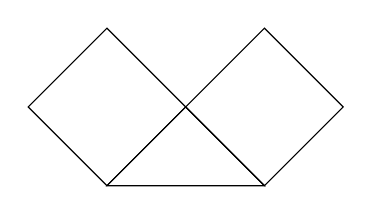
\begin{tikzpicture}
    % Définition des sommets du triangle rectangle isocèle
    \coordinate (A) at (0,0);
    \coordinate (B) at (2,0);
    \coordinate (C) at (1,1);
    
    % Tracé du triangle
    \draw (A) -- (B) -- (C) -- cycle;
    
    % Carré sur le côté AC
    \coordinate (D) at (-1,1);
    \coordinate (E) at (0,2);
    \draw (A) -- (D) -- (E) -- (C) -- cycle;

    % Carré sur le côté BC
    \coordinate (F) at (3,1);
    \coordinate (G) at (2,2);
    \draw (B) -- (F) -- (G) -- (C) -- cycle;
\end{tikzpicture}
\end{center}


\hfill\break
\hrule
\hfill\break

\newpage


\exo[3]{Plaque Gros Trou}

On considère la plaque homogène ci-dessous.

\begin{center}
    
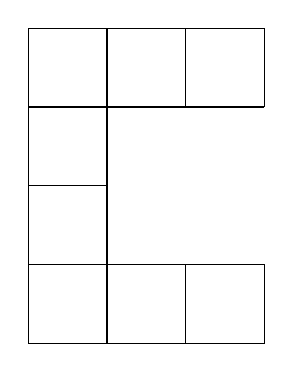
\begin{tikzpicture}
    % Dessiner la grille complète de 3x4
    \foreach \x in {0,1,2}
        \foreach \y in {0,1,2,3}
            \draw (\x,\y) rectangle (\x+1,\y+1);

    % Supprimer deux carrés sur le côté droit (en ne les dessinant pas)
    %\fill[white] (2,1) rectangle (3,2); % Efface le carré en (2,1)
    %\fill[white] (2,2) rectangle (3,3); % Efface le carré en (2,2)
        \fill[white] (1,1) rectangle (3,3); % Efface le carré en (2,1)
    %\fill[white] (1,2) rectangle (3,3); % Efface le carré en (2,2)

    % Redessiner les lignes pour éviter que les coins disparaissent
    \draw(2,0) -- (2,1);
    \draw (1,1) -- (1,3);
      \draw (1,1) -- (3,1);
   
     \draw(0,3)--(3,3);
      \draw[white](3,1)--(3,3);
\end{tikzpicture}

\end{center}
 Déterminer la position de son centre d'inertie et le placer sur la figure avec une précision acceptable.
 
\hfill\break
\hrule
\hfill\break

\exo[3]{Plaque Petit Trou}
On considère la plaque homogène ci-dessous.

\begin{center}
    
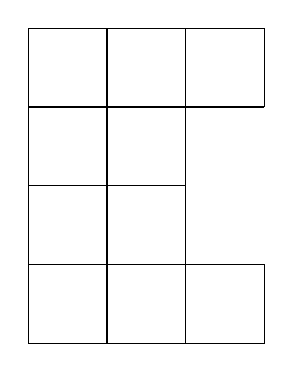
\begin{tikzpicture}
    % Dessiner la grille complète de 3x4
    \foreach \x in {0,1,2}
        \foreach \y in {0,1,2,3}
            \draw (\x,\y) rectangle (\x+1,\y+1);

    % Supprimer deux carrés sur le côté droit (en ne les dessinant pas)
    \fill[white] (2,1) rectangle (3,2); % Efface le carré en (2,1)
    \fill[white] (2,2) rectangle (3,3); % Efface le carré en (2,2)

    % Redessiner les lignes pour éviter que les coins disparaissent
    \draw (2,0) -- (2,4);
    \draw (2,3) -- (3,3);
    \draw (2,1) -- (3,1);
    \draw[white](3,1)--(3,3);
    \draw[white](2, 2) -- (3, 2);
\end{tikzpicture}

\end{center}
 Déterminer la position de son centre d'inertie et le placer sur la figure avec une précision acceptable.





%%%%%


\end{document}